\documentclass[14pt]{beamer} %Makes presentation
%\documentclass[handout]{beamer} %Makes Handouts
\usetheme{Singapore} %Gray with fade at top
\useoutertheme[subsection=false]{miniframes} %Supppress subsection in header
\useinnertheme{rectangles} %Itemize/Enumerate boxes
\usecolortheme{seagull} %Color theme
\usecolortheme{rose} %Inner color theme

\definecolor{light-gray}{gray}{0.75}
\definecolor{dark-gray}{gray}{0.55}
\setbeamercolor{item}{fg=light-gray}
\setbeamercolor{enumerate item}{fg=dark-gray}

\setbeamertemplate{navigation symbols}{}
%\setbeamertemplate{mini frames}[default]
\setbeamercovered{dynamics}
\setbeamerfont*{title}{size=\Large,series=\bfseries}

%\setbeameroption{notes on second screen} %Dual-Screen Notes
%\setbeameroption{show only notes} %Notes Output

\setbeamertemplate{frametitle}{\vspace{.5em}\bfseries\insertframetitle}
\newcommand{\heading}[1]{\noindent \textbf{#1}\\ \vspace{1em}}

\usepackage{bbding,color,multirow,times,ccaption,tabularx,graphicx,verbatim,booktabs,fixltx2e}
\usepackage{colortbl} %Table overlays
\usepackage[english]{babel}
\usepackage[latin1]{inputenc}
\usepackage[T1]{fontenc}
\usepackage{lmodern}

%\author[]{Thomas J. Leeper}
\institute[]{
  \inst{}%
  Department of Political Science and Government\\Aarhus University
}

\usepackage{tikz}
\usepackage{pbox}
\usetikzlibrary{calc}
\usetikzlibrary{shapes}
\usetikzlibrary{arrows}
\usetikzlibrary{shapes.multipart}
\usetikzlibrary{matrix}
\usetikzlibrary{positioning}

\title{Practical Data Issues}

\date[]{March 3, 2015}

\begin{document}

\frame{\titlepage}

\frame{\tableofcontents}


\section{Data Transformations}
\frame{\tableofcontents[currentsection]}

\frame{
	\frametitle{Tidy Data Activity}
	\begin{itemize}\itemsep2em
	\item Construct the data described on the worksheet into a rectangular dataset
	\item You can use Stata's data editor, Excel, a Word table, etc.
	\item You have 7 minutes
	\end{itemize}
}

\frame{
	\frametitle{Data Formats}
	\begin{itemize}\itemsep1em
		\item A dataset is a rectangular matrix of:
			\begin{itemize}
				\item Observations (rows)
				\item Variables (columns)
			\end{itemize}
		\item But what counts as an observation?
			\begin{itemize}
				\item<1-> Countries, by year
				\item<2-> Dyads (e.g., couples, neighboring countries)
				\item<3-> Candidates, by election
			\end{itemize}
	\end{itemize}
}


\frame{
	\frametitle{Data in Wide Format}
	\begin{center}
		\begin{tabular}{lrrrr}
			Country     & \pbox{20cm}{GDP\\2012} & \pbox{20cm}{GDP\\2013} & \pbox{20cm}{Life\\Expectancy\\2012} & \pbox{20cm}{L.E.\\2013} \\ \hline
			Afghanistan &           20.5 &           20.3 &                     60 &          61 \\
			Albania     &           12.3 &           12.9 &                     77 &          77 \\
			Algeria     &          204.3 &          210.2 &                     71 &          71 \\
			Angola      &          114.3 &          124.2 &                     51 &          51 \\ \hline
		\end{tabular}
	\end{center}
}


\frame{
	\frametitle{Data in Long Format}
	\begin{center}
		\begin{tabular}{llrr}
			Country     & Year & GDP (\$B) & Life Expectancy \\ \hline
			Afghanistan & 2012 &      20.5 &              60 \\
			Afghanistan & 2013 &      20.3 &              61 \\
			Albania     & 2012 &      12.3 &              77 \\
			Albania     & 2013 &      12.9 &              77 \\
			Algeria     & 2012 &     204.3 &              71 \\
			Algeria     & 2013 &     210.2 &              71 \\
			Angola      & 2012 &     114.3 &              51 \\
			Angola      & 2013 &     124.2 &              51 \\ \hline
		\end{tabular}
	\end{center}
}

\frame{
	\frametitle{Wide and Long in Stata}
	\begin{itemize}\itemsep1em
		\item When data are cross-sectional, there is only wide
		\item When data have other forms, they can be represented in multiple ways
		\item Next week we'll start discussing over-time data
		\item In most case, we need data in \textbf{long} or ``tidy'' format
		\item In Stata, this will require the \textbf{reshape} and \textbf{xtset} commands
	\end{itemize}
}

% data cleaning


% data merging
\frame{
	\frametitle{Merging Multiple Datasets}
	\begin{itemize}\itemsep1em
	\item We can only analyze one dataset at a time
	\item All data about our observations needs to be in one file
	\item Often we need data from multiple files together
	\item To use them, we need to merge
	\end{itemize}
}

\frame{
	\frametitle{Four Ways of Merging Data}
	\begin{enumerate}\itemsep2em
	\item 1:1
	\item 1:many 
	\item many:1
	\item many:many
	\end{enumerate}
}

% graphs of different join relationships

\begin{frame}[fragile]
	\frametitle{1:1 Merging}
	\small
	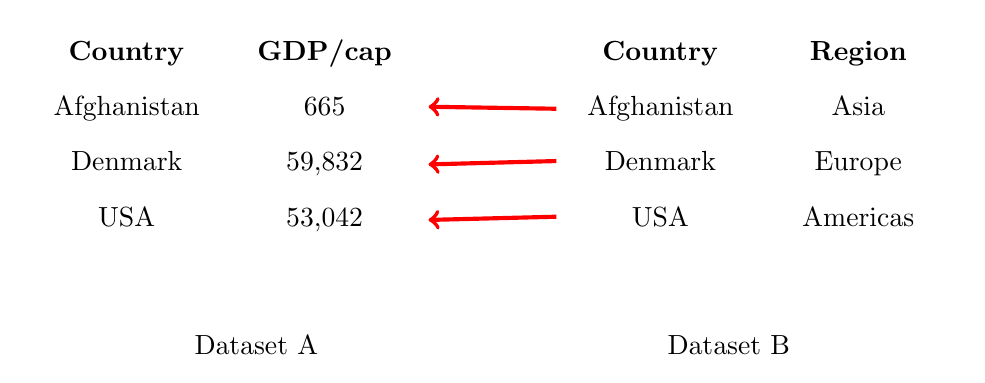
\begin{tikzpicture}[scale=0.8,every node/.style={inner sep=0,outer sep=2pt}]
	\matrix (A) [matrix of nodes,row sep = 0cm, nodes={draw = white, minimum size=.65cm, text width=2.5cm,align=center}] at (0,1) {
	\textbf{Country} & \textbf{GDP/cap} &[1.75cm] \textbf{Country} & \textbf{Region} \\
	Afghanistan & 665 & Afghanistan & Asia \\
	Denmark & 59,832 & Denmark & Europe\\
	USA & 53,042 & USA & Americas\\
	};
	
	\draw[->,red,line width = 1.5] (A-2-3.west) -- (A-2-2.east);
	\draw[->,red,line width = 1.5] (A-3-3.west) -- (A-3-2.east);
    \draw[->,red,line width = 1.5] (A-4-3.west) -- (A-4-2.east);
	\node (C) [below=of A, xshift=-3cm]{Dataset A};
	\node (D) [below=of A, xshift=3cm]{Dataset B};
	\end{tikzpicture}
\end{frame}

\begin{frame}[fragile]
	\frametitle{1:many Merging}
	\small
	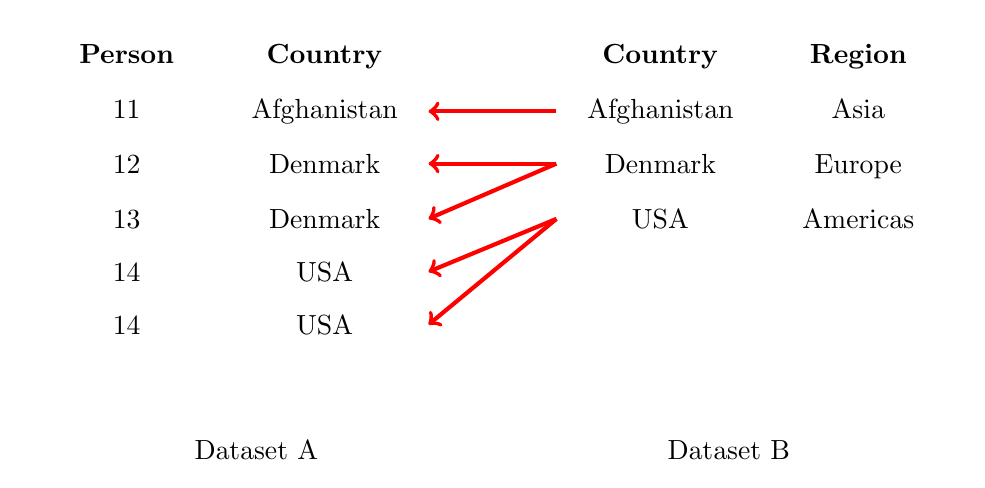
\begin{tikzpicture}[scale=0.8,every node/.style={inner sep=0,outer sep=2pt}]
	\matrix (A) [matrix of nodes,row sep = 0cm, nodes={draw = white, minimum size=.65cm, text width=2.5cm,align=center}] at (0,1) {
	\textbf{Person} & \textbf{Country} &[1.75cm] \textbf{Country} & \textbf{Region} \\
	11 & Afghanistan & Afghanistan & Asia \\
	12 & Denmark & Denmark & Europe\\
	13 & Denmark & USA & Americas\\
    14 & USA & \\
    14 & USA & \\
	};
	
	\draw[->,red,line width = 1.5] (A-2-3.west) -- (A-2-2.east);
	\draw[->,red,line width = 1.5] (A-3-3.west) -- (A-3-2.east);
    \draw[->,red,line width = 1.5] (A-3-3.west) -- (A-4-2.east);
    \draw[->,red,line width = 1.5] (A-4-3.west) -- (A-5-2.east);
	\draw[->,red,line width = 1.5] (A-4-3.west) -- (A-6-2.east);
	\node (C) [below=of A, xshift=-3cm]{Dataset A};
	\node (D) [below=of A, xshift=3cm]{Dataset B};
	\end{tikzpicture}
\end{frame}

\begin{frame}[fragile]
	\frametitle{many:1 Merging}
	\small
	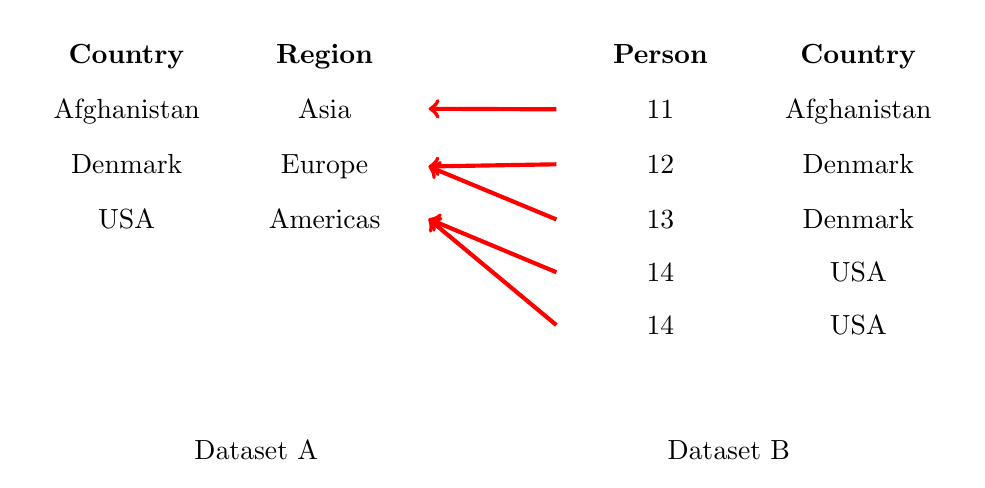
\begin{tikzpicture}[scale=0.8,every node/.style={inner sep=0,outer sep=2pt}]
	\matrix (A) [matrix of nodes,row sep = 0cm, nodes={draw = white, minimum size=.65cm, text width=2.5cm,align=center}] at (0,1) {
	\textbf{Country} & \textbf{Region} &[1.75cm] \textbf{Person} & \textbf{Country} \\
	Afghanistan & Asia & 11 & Afghanistan \\
	Denmark & Europe & 12 & Denmark \\
	USA & Americas & 13 & Denmark \\
    & & 14 & USA & \\
    & & 14 & USA & \\
	};
	
	\draw[->,red,line width = 1.5] (A-2-3.west) -- (A-2-2.east);
	\draw[->,red,line width = 1.5] (A-3-3.west) -- (A-3-2.east);
    \draw[->,red,line width = 1.5] (A-4-3.west) -- (A-3-2.east);
    \draw[->,red,line width = 1.5] (A-5-3.west) -- (A-4-2.east);
	\draw[->,red,line width = 1.5] (A-6-3.west) -- (A-4-2.east);
	\node (C) [below=of A, xshift=-3cm]{Dataset A};
	\node (D) [below=of A, xshift=3cm]{Dataset B};
	\end{tikzpicture}
\end{frame}

% Stata's `merge` command

\frame{
	\frametitle{Questions about merging?}
}

\frame{
	\frametitle{Aggregating Observations}
	\begin{itemize}\itemsep1em
	\item Our data are not always available on the unit of analysis we need
	\item For example, we might have multiple observations (rows) for a given unit and we need to create a dataset that just has one observation (row) for each unit
	\item Examples?
	\item<2-> How do we do this?
	\end{itemize}
}

\begin{frame}[fragile]
	\frametitle{Aggregating Observations}
	\small
	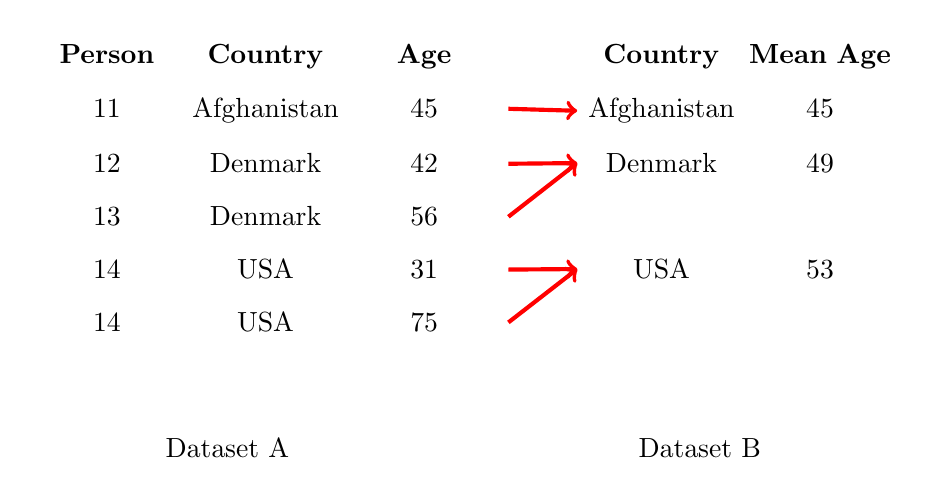
\begin{tikzpicture}[scale=0.8,every node/.style={inner sep=0,outer sep=2pt}]
	\matrix (A) [matrix of nodes,row sep = 0cm, nodes={draw = white, minimum size=.65cm, text width=2cm,align=center}] at (0,1) {
	\textbf{Person} & \textbf{Country} & \textbf{Age} &[1cm] \textbf{Country} & \textbf{Mean Age} \\
	11 & Afghanistan & 45 & Afghanistan & 45\\
	12 & Denmark & 42 & Denmark & 49\\
	13 & Denmark & 56 \\
    14 & USA & 31 & USA & 53 \\
    14 & USA & 75 \\
	};
	
	\draw[->,red,line width = 1.5] (A-2-3.east) -- (A-2-4.west);
	\draw[->,red,line width = 1.5] (A-3-3.east) -- (A-3-4.west);
    \draw[->,red,line width = 1.5] (A-4-3.east) -- (A-3-4.west);
    \draw[->,red,line width = 1.5] (A-5-3.east) -- (A-5-4.west);
	\draw[->,red,line width = 1.5] (A-6-3.east) -- (A-5-4.west);
	\node (C) [below=of A, xshift=-3cm]{Dataset A};
	\node (D) [below=of A, xshift=3cm]{Dataset B};
	\end{tikzpicture}
\end{frame}

% Stata's `collapse` command


% scaling and reliability


\frame{
	\frametitle{Scale Constructions}
	\begin{itemize}\itemsep1em
	\item Scale construction is the act of aggregating multiple variables into a smaller number of variables
	\item Two advantages:
		\begin{itemize}
		\item Reducing measurement error
		\item Avoiding collinearity
		\end{itemize}
	\item Examples
		\begin{itemize}
		\item<2-> 
		\item<3-> Others
		\end{itemize}
	\end{itemize}
}


\frame{
	\frametitle{Cronbach's $\alpha$}
	\begin{itemize}\itemsep1em
	\item Scaling only makes sense if variables ``go together''
		\begin{itemize}
		\item We can assess them \textit{pairwise} by looking at correlations between variables
		\item But it's helpful to have a way to assess the scale as a whole
		\end{itemize}
	\item Definition:
		$\alpha = \dfrac{ N \bar{c} }{ \bar{v} + (N-1) \bar{c} }$
		\begin{itemize}
		\item N: number of items
		\item $\bar{c}$: average covariance of items
		\item $\bar{v}$: average variance of items
		\end{itemize}
	\end{itemize}
}


\begin{frame}[fragile]
\frametitle{Cronbach's $\alpha$ in Stata I}
\footnotesize
\begin{verbatim}
. corr price headroom trunk weight length, cov
(obs=45)

             |    price headroom    trunk   weight   length
-------------+---------------------------------------------
       price |  7.7e+06
    headroom |  511.298  .718434
       trunk |  3793.78  2.78662  20.4343
      weight |  1.2e+06  395.896  2544.42   658519
      length |  28383.1  12.5265  79.5833  18332.8  561.391

\end{verbatim}
\end{frame}

\begin{frame}[fragile]
\frametitle{Cronbach's $\alpha$ in Stata II}
\scriptsize
\begin{columns}
\column{\dimexpr\paperwidth-25pt}
\begin{verbatim}
. alpha price headroom trunk weight length, item

Test scale = mean(unstandardized items)

                                                            average
                             item-test     item-rest       interitem
Item         |  Obs  Sign   correlation   correlation     covariance      alpha
-------------+-----------------------------------------------------------------
price        |   70    +       0.9360        0.2201        3120.148      0.0854
headroom     |   66    +       0.2471        0.2453        182861.2      0.2626
trunk        |   69    +       0.3928        0.3752        186996.9      0.2649
weight       |   64    +       0.5665        0.3710        5565.038      0.0106
length       |   69    +       0.5604        0.5414        180695.7      0.2578
-------------+-----------------------------------------------------------------
Test scale   |                                             111565.7      0.2483
-------------------------------------------------------------------------------
\end{verbatim}
\end{columns}
\end{frame}


\frame{
	\frametitle{Other forms of scaling}
	\begin{itemize}
	\item<2-> IRT Models
	\item<3-> Factor Analysis
	\item<4-> Principal Components Analysis
	\vspace{1em}
	\item<5-> We are not discussing these here
	\item<5-> You can achieve them in Stata's SEM module
	\end{itemize}
}



\section{Data Gathering}
\frame{\tableofcontents[currentsection]}

\frame{
	\frametitle{}
}


\section{Missing Data}
\frame{\tableofcontents[currentsection]}


\frame{
	\frametitle{Missing Data Ideal World}
	\begin{itemize}\itemsep1em
	\item Everything we've talked about assumes no missingness
	\item We always assume that we have a representative sample of i.i.d. data
	\item We analyze all of our data as is
	\end{itemize}
}

\frame{
	\frametitle{Missing Data}
	\begin{itemize}\itemsep1em
	\item What is it?
	\item<2-> Why are data missing?
	\item<3-> How often do we encounter missing data?
	\end{itemize}
}

\frame{
	\frametitle{Does Missingness Matter?}
	\small
	\begin{quote}
	If the data are missing at random, then the size of the random sample available from the population is simply reduced. Although this makes the estimators less precise, it does not introduce any bias [\dots] There are ways to use the information on observations where only some variables are missing, but this is not often done in practice. The improvement in the estimators is usually slight, while the methods are somewhat complicated. In most cases, we just ignore the observations that have missing information. (Wooldridge 2013, 314)
	\end{quote}

}

\frame{
	\frametitle{Missing Data in Practice}
	\begin{itemize}\itemsep1em
	\item Often have missing data for a variety of reasons
	\item We often don't realize we have missing data
	\item Missing data can be problematic (but not always)
	\item Stata handles missingness through \textbf{complete case} or \textbf{available case} analysis
	\end{itemize}
}

\frame{
	\frametitle{Complete/Available Cases}
	\begin{itemize}\itemsep1em
	\item \textbf{Complete case analysis} involves subsetting a dataset to retain only observations that are complete on all variables before any analysis
	\item \textbf{Available case analysis} involves dynamically subsetting a dataset to retain only observations that are complete on all variables used in a given analysis
		\begin{itemize}
		\item Sometimes also called \textit{case-wise deletion} or \textit{list-wise deletion}
		\end{itemize}
	\item<2-> Do we use either of these techniques?
	\end{itemize}
}

\frame{
	\frametitle{Impacts of Missingness}
	\begin{enumerate}\itemsep1em
	\item Scale construction problems
	\item Statistical efficiency
	\item Representativeness (External validity)
	\item Comparability of subsample analyses
	\item Causal inference
	\end{enumerate}
}

\frame{
	\frametitle{Possible Impact 1: Scales}
	\begin{itemize}\itemsep1em
	\item It is common to analyze variables constructed as scales
		\begin{itemize}
		\item Simple additive scales being the most common
		\end{itemize}
	\item Examples?
		\begin{itemize}
		\item Political knowledge
		\item Frequency of voting
		\item Democracy
		\item Budgets across multiple domains
		\end{itemize}
	\end{itemize}
}

\frame{
	\frametitle{A Simple Example}
	\begin{center}
    \begin{tabular}{lllll} \hline
    Case & Item 1 & Item 2 & Item 3 & Sum \\ \hline
    A & 1 & 2 & 1 & ? \\ \hline
    B & 1 & . & 3 & ? \\ \hline
    C & . & 1 & 1 & ? \\ \hline
    D & 2 & 1 & 2 & ? \\ \hline
    E & 1 & . & . & ? \\ \hline
    F & . & . & . & ? \\ \hline
    \end{tabular}
    \end{center}
}

\frame{
	\frametitle{Possible Impact 1: Scales}
	\begin{itemize}\itemsep2em
	\item When constructing multi-item scales, we need to know how to deal with missingness
	\item Stata's default is to coerce missingness to zero
	\item Another strategy is \textit{imputation}
	\end{itemize}
}


\frame{
	\frametitle{Possible Impact 2: Efficiency}
	\begin{itemize}\itemsep1em
	\item Recall: $Var(\hat{\beta}) = \hat{\sigma} (\mathbf{X}'\mathbf{X})^{-1}$
	\item And $\hat{\sigma}^2 = \frac{SSR}{n-2}$, so that $\hat{\sigma} = \frac{\sqrt{SSR}}{\sqrt{n-2}}$
	\item As sample size increases we gain precision
	\item Missing data reduces our \textit{effective sample size} for analysis
	\end{itemize}
}

\frame{
	\begin{center}
   	\begin{tikzpicture}[scale=2]
 	  \draw[->] (0,0) -- (5,0) node[right] {$n$};
 	  \draw[->] (0,0) -- (0,3) node[above] {$\hat{\sigma}$};
 	  \draw[domain=0.1:5,smooth,variable=\x,blue,thick] plot ({\x},{1/sqrt(\x)});
 	  \draw[->,thick] (1.5,2.5) node[right] {This matters most when $n$ is small} -- (0.5,1.5);
   	\end{tikzpicture}
   	\end{center}
}

\frame{
	\frametitle{Possible Impact 3: Representativeness}
	\begin{itemize}\itemsep1em
	\item Recall: We generally try to make inferences from sample to a well-specified population
	\item If missingness is \textit{completely} random, we simply have a smaller sample
	\item If missingness is not \textit{completely} random, we no longer have a representative sample
		\begin{itemize}
		\item This means we our sample estimates are biased
		\end{itemize}
	\end{itemize}
}

\frame{
	\frametitle{Possible Impact 4: Comparability}
	\begin{itemize}\itemsep1em
	\item When there is missingness, we (and Stata) default to \textit{available case analysis}
	\item Our analyses might be based on different subsamples of our data
	\item Thus the precision of our estimates from different analyses might vary
	\item Can be solved through \textit{complete case analysis}
	\end{itemize}
}

\frame{
	\frametitle{Possible Impact 5: Causal Inference}
	\begin{itemize}\itemsep1em
	\item Our inferences might be biased if missingness is caused by a third variable
	\item This is especially bad if the third variable is also causally important for our outcome
	\end{itemize}
}


\frame[label=causalgraph]{
   	\begin{center}
   	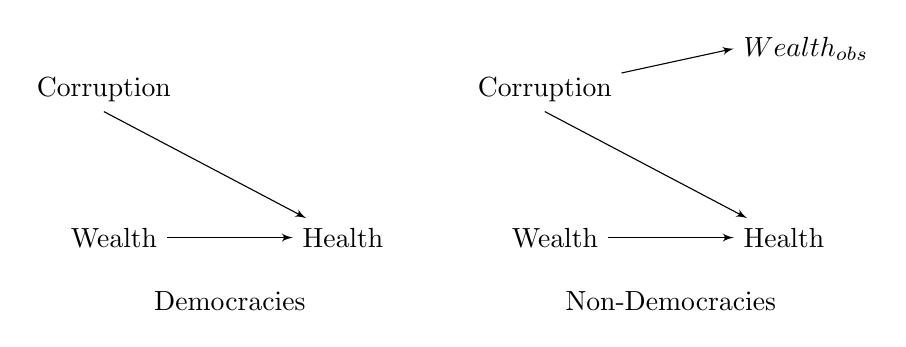
\begin{tikzpicture}[scale=0.8,>=latex',circ/.style={draw, shape=circle, node distance=5cm, line width=1.5pt}]
        \draw[->] (0,0) node[left] (X1) {Wealth} -- (2,0) node[right] (Y1) {Health};
        \draw[->] (-1,2) node[above] (Z1) {Corruption} -- (Y1);
        \draw (1,-1) node (Democracy) {Democracies};

        \draw[->] (7,0) node[left] (X2) {Wealth} -- (9,0) node[right] (Y2) {Health};
        \draw[->] (6,2) node[above] (Z2) {Corruption} -- (Y2);
        \draw[->] (Z2) -- (9,3) node[right] (Yobs) {$Wealth_{obs}$};
        \draw (8,-1) node (non) {Non-Democracies};
    \end{tikzpicture}
    \end{center}
}

\frame{
	\frametitle{Impact of Missingness Depends on \textit{Why} Data Are Missing}
	\begin{itemize}\itemsep2em
	\item Missing Completely At Random (MCAR)
	\item Missing At Random
	\item Missing Not At Random (MNAR)
	\end{itemize}
}

\section{MCAR}
\frame{\tableofcontents[currentsection]}

\frame{
	\frametitle{MCAR/Ignorable}
    \begin{itemize}\itemsep1em
    \item Best-case scenario
    \item Our data constitute a representative subsample of our sample, making it a representative sample of our population
	\item Examples?
		\begin{itemize}
		\item<2-> We obtain a complete sample but randomly analyze only part of it
		\item<3-> Survey respondents randomly assigned to different questionnaires
		\end{itemize}
    \item<4-> How do we deal with missingness?
    	\begin{itemize}
    	\item<5-> We can probably ignored it
    	\end{itemize}
    \end{itemize}
}

\frame{
	\frametitle{Impacts of Missingness (MCAR)}
	\begin{enumerate}\itemsep1em
	\item \alert{Scale construction problems}
	\item \alert{Statistical efficiency}
	\item \color{gray}{Representativeness (External validity)}
	\item \color{gray}{Comparability of subsample analyses}
	\item \color{gray}{Causal inference}
	\end{enumerate}
}


\section{MAR}
\frame{\tableofcontents[currentsection]}

\frame{
	\frametitle{MAR}
    \begin{itemize}\itemsep1em
    \item Middle-ground scenario
    \item Data are missing for a (non-random) reason that we understand and observe
    \item Missingness is \textbf{\textit{conditionally} ignorable}
    \end{itemize}
}

\frame[label=causalgraph2]{
   	\begin{center}
   	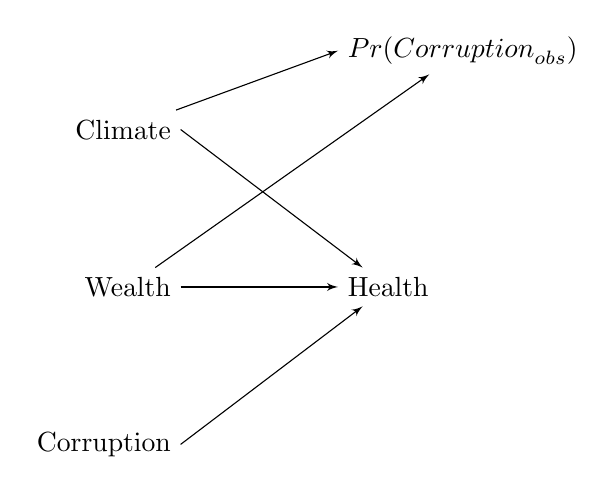
\begin{tikzpicture}[>=latex',circ/.style={draw, shape=circle, node distance=5cm, line width=1.5pt}]
        \draw[->] (0,0) node[left] (X1) {Wealth} -- (2,0) node[right] (Y1) {Health};
        \draw[->] (0,2) node[left] (Z1) {Climate} -- (Y1);
        \draw[->] (0,-2) node[left] (W1) {Corruption} -- (Y1);
        \draw[->] (Z1) -- (2,3) node[right] (Xobs) {$Pr(\text{Corruption}_{obs})$};
        \draw[->] (X1) -- (Xobs);
    \end{tikzpicture}
    \end{center}
}


\frame{
	\frametitle{Impacts of Missingness (MAR)}
	\begin{enumerate}\itemsep1em
	\item \alert{Scale construction problems}
	\item \alert{Statistical efficiency}
	\item \color{gray}{Representativeness (External validity)}
	\item \alert{Comparability of subsample analyses}
	\item \color{gray}{Causal inference}
	\end{enumerate}
}


\frame{
	\frametitle{Handling MAR Data}
	\begin{itemize}\itemsep1em
	\item Regression adjustment
	\item Reweighting
	\item Single imputation
		\begin{itemize}
		\item Several possible methods
		\end{itemize}
	\item Multiple imputation
		\begin{itemize}
		\item Several possible methods
		\end{itemize}
	\end{itemize}
}

\frame{
	\frametitle{Regression adjustment}
	\begin{itemize}\itemsep1em
	\item 
	\end{itemize}
}

\frame{
	\frametitle{Weighting adjustments}
	\begin{itemize}\itemsep1em
	\item Stratify the sample based on observed characteristics, where the proportion of the \textit{population} in each stratum is also known
	\item Reweight each observation so sample matches population distributions
	\item Essentially, over-weight observed cases from strata where there are missing values
	\item Several variants of this:
		\begin{itemize}
		\item Weighting classes
		\item Post-stratification
		\item Raking
		\end{itemize}
	\end{itemize}
}


\frame{
	\frametitle{Single imputation}
	\begin{itemize}\itemsep1em
	\item Fill in missing values with an \textit{imputed} value
	\item Several different methods, including:
		\begin{itemize}
		\item Zero
		\item Mean value
		\item Random value
		\item Inferred value
		\item Hot-Deck imputation
		\item Regression imputation
		\end{itemize}
	\end{itemize}
}

\frame{
	\frametitle{Single Imputation I}
	\begin{itemize}\itemsep1em
	\item<1-> Zero: Will bias results, unless $\bar{X} = 0$
	\item<2-> Mean: Unbiased\dots why?
	\item<3-> Random: Unbiased\dots why?
	\item<4-> Inferred
		\begin{itemize}
		\item Uses observed data to guess at missing value
		\item Could be historical records, logic, etc.
		\end{itemize}
	\end{itemize}
}

\frame{
	\frametitle{Single Imputation I}
	\begin{itemize}\itemsep1em
		\item Hot-Deck Imputation
			\begin{enumerate}
			\item<1-> Sort dataset by all complete variables
			\item<2-> For every missing value, carry forward last observed value
			\item<3-> Imputations depend on sort order
			\end{enumerate}
		\item Regression Imputation
			\begin{itemize}
			\item<4-> Regress partially observed variable on all complete variables
			\item<5-> Replace missing value with fitted value $\hat{y}$ from regression
			\item<6-> Imputations depend on model
			\item<7-> Can dramatically overstate certainty unless a stochastic component is added
			\end{itemize}
	\end{itemize}
}


\frame{
	\frametitle{Multiple Imputation}
	\begin{itemize}\itemsep1em
	\item Apply a stochastic single imputation technique multiple times and merge the results of the analysis performed on each imputed dataset
		\begin{itemize}
		\item Usually some form of regression imputation
		\end{itemize}
	\item Attempts to account for uncertainty due to imputation
		\begin{itemize}
		\item Single imputation overstates our certainty
		\end{itemize}
	\end{itemize}
}

\frame{
	\frametitle{MI Procedure}
	\begin{enumerate}\itemsep1em
	\item Impute missing values and estimate $\hat{\beta}_m$
	\item Repeat for all $M$ datasets
	\item Aggregate results: $\hat{\beta} = \frac{1}{M}\sum_{m=1}^{M} \hat{\beta}_m$
	\item Account for missingness when estimating variance:
		\begin{itemize}\itemsep0.5em
		\item $\text{Within} = \frac{1}{m}\sum_1^M Var(\hat{\beta}_m)$
		\item $\text{Between} = \frac{1}{m-1} \sum_1^M (\hat{\beta}_m - \hat{\beta})^2$
		\item $Var(\hat{\beta}) = \text{Within} + (1 + \frac{1}{m}) \text{Between}$
		\end{itemize}
	\end{enumerate}
}

\frame{
	\frametitle{An Example I}
	\begin{itemize}\itemsep1em
	\item What is the effect of university education on an individuals' political tolerance?
	\item Missingness in various covariates
	\item Multiply impute missing values
	\item On each imputed dataset, we estimate:\\
		$\text{Tolerance} = \beta_0 + \beta_1 \text{Education} + \beta_{2...k} \text{Controls}$
	\item Our test statistic is $\hat{\beta}_{\text{Education}}$
	\end{itemize}
}

\frame{
	\frametitle{An Example II}
	\begin{center}
	\begin{tabular}{llll}\hline
	Dataset & $\hat{\beta}_{\text{Education}}$ & $SE_{\hat{\beta}}$ & $Var(\hat{\beta})$ \\ \hline
	1 & 4.32 & 0.95 & 0.9025 \\
	2 & 4.15 & 1.16 & 1.3456 \\
	3 & 4.86 & 0.83 & 0.6889 \\
	4 & 3.98 & 1.04 & 1.0816 \\
	5 & 4.50 & 0.91 & 0.8281 \\ \hline
	\end{tabular}
	
	\vspace{2em}
	\onslide<2->{$\hat{\beta}_{Overall} = \frac{4.32 + 4.15 + 4.86 + 3.98 + 4.50}{5} = 4.362$}
	\end{center}
}


\frame{
	\frametitle{An Example III}
	\small
	\begin{align*}
	\onslide<1->{Var_{\text{W}} & = \frac{1}{5} (0.9025 + 1.3456 + 0.6889 + 1.0816 + 0.8281)}\\
		\onslide<2->{& = \frac{4.8467}{5} = 0.96934}\\[1em]
	\onslide<3->{Var_{\text{B}} & = \frac{1}{m-1}(-0.042^2 + 0.212^2 + 0.498^2 + -0.382^2 + 0.138^2)}\\
		\onslide<4->{& = \frac{0.45968}{4} = 0.11492}\\[1em]
	\onslide<5->{Var(\hat{\beta}) & = W + (1 + \frac{1}{m}) B = 1.107244}\\[1em]
	\onslide<7->{SE(\hat{\beta}) & = \sqrt{1.107244} = 1.052257}
	\end{align*}
}

\frame{
	\frametitle{MAR: Conclusion}
	\begin{itemize}\itemsep1em
	\item<1-> If we assume MAR, lots of available strategies
	\item<2-> Added value of imputation depends on scale of missingness and assumptions
	\item<3-> Can overstate our certainty about model estimates
	\item<4-> Can introduce measurement error if we misunderstand the pattern of missingness, which then leads to bias
	\end{itemize}
}

\section{MNAR}
\frame{\tableofcontents[currentsection]}

\frame{
	\frametitle{MNAR}
    \begin{itemize}\itemsep1em
    \item Worst-case scenario
    \item Missingness is \textbf{non-ignorable}
    \item Data are missing due to factors that are in our model
    \item Examples?
    	\begin{itemize}
    	\item<2-> Survey participation based on topic
    	\item<3-> Income reporting based on income
    	\end{itemize}
    \end{itemize}
}

\frame[label=mnar]{
	\frametitle{MNAR: Special Cases}
    \begin{enumerate}\itemsep2em
    \item Truncation (Sample selection bias)
    \item Censoring
    \end{enumerate}
}

\frame[label=causalgraph3]{
   	\begin{center}
   	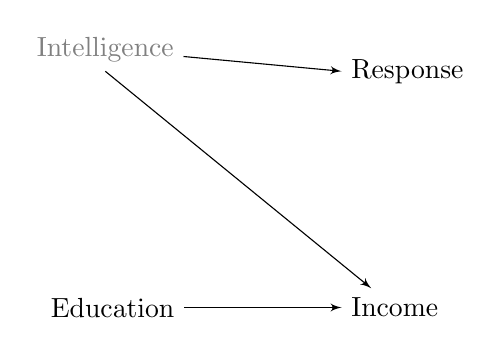
\begin{tikzpicture}[>=latex',circ/.style={draw, shape=circle, node distance=5cm, line width=1.5pt}]
        \draw[->] (0,0) node[left] (X1) {Education} -- (2,0) node[right] (Y1) {Income};
        \draw[->] (-1,3) node[above] (Z1) {\color{gray}{Intelligence}} -- (Y1);
        %\draw[->] (Z1) -- (X1);
        \draw<2->[->] (Z1) -- (2,3) node[right] (Yobs) {Response};
    \end{tikzpicture}
    \end{center}
}

% not a problem if Z not associated with Y
% can also have omitted variable bias if Z causes X

\frame{
	\begin{center}
   	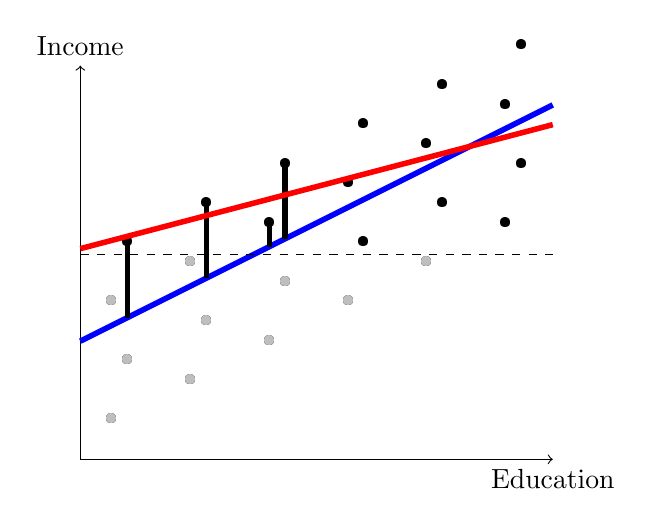
\begin{tikzpicture}
 	  \draw[->] (0,0) -- (6,0) node[below] {Education};
 	  \draw[->] (0,0) -- (0,5) node[above] {Income};
	  \foreach \Point in
	    {(0.4,0.50), (0.6,1.25), (0.4,2.00), (0.6,2.75),
	     (1.4,1.00), (1.6,1.75), (1.4,2.50), (1.6,3.25),
	     (2.4,1.50), (2.6,2.25), (2.4,3.00), (2.6,3.75),
	     (3.4,2.00), (3.6,2.75), (3.4,3.50), (3.6,4.25),
	     (4.4,2.50), (4.6,3.25), (4.4,4.00), (4.6,4.75),
	     (5.4,3.00), (5.6,3.75), (5.4,4.50), (5.6,5.25)}{
	      \node at \Point {\textbullet};
	  };
	  \draw[blue,line width=2pt] (0.00,1.5) -- (6.00,4.50);
	  \draw<2->[dashed] (0.00,2.60) -- (6.00,2.60);
	  \foreach \Point in
        {(0.4,0.50), (0.6,1.25), (0.4,2.00), (1.4,1.00), (1.4,2.50), 
         (1.6,1.75), (2.4,1.50), (2.6,2.25), (3.4,2.00), (4.4,2.50)}{
         \node<2->[lightgray] at \Point {\textbullet};
	  	  };
	  \draw<3>[line width=2pt] (0.6,1.80) -- (0.6,2.75);
	  \draw<3>[line width=2pt] (1.6,2.30) -- (1.6,3.25);
	  \draw<3>[line width=2pt] (2.4,2.70) -- (2.4,3.00);
	  \draw<3>[line width=2pt] (2.6,2.80) -- (2.6,3.75);
	  \draw<4->[red, line width=2pt] (0.00,2.675) -- (6.00,4.25);
   	\end{tikzpicture}
   	\end{center}
}


\frame{
	\frametitle{Sample Selection Bias}
	\begin{itemize}\itemsep1em
	\item Whether we observe a unit depends on factors related to $X$ and $Y$
	\item Common analytic strategy: Heckman Models
		\begin{itemize}
		\item OLS with an additional covariate
		\item Regress missingness on variable(s) \textit{not} in our main model
		\item Include predicted probability of observing case as a covariate in main model
		\end{itemize}
	\item<2-> Examples?
		\begin{itemize}
		\item<3-> Effect of grades on job performance
		\item<4-> Systematic survey nonresponse
		\end{itemize}
	\end{itemize}
}

\againframe{mnar}

\frame[label=causalgraph4]{
   	\begin{center}
   	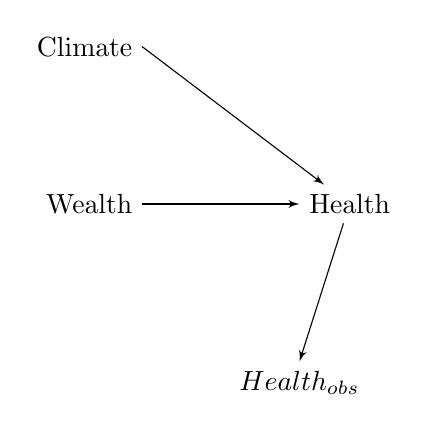
\begin{tikzpicture}[>=latex',circ/.style={draw, shape=circle, node distance=5cm, line width=1.5pt}]
        \draw[->] (0,0) node[left] (X1) {Wealth} -- (2,0) node[right] (Y1) {Health};
        \draw[->] (0,2) node[left] (Z1) {Climate} -- (Y1);
        \draw[->] (Y1) -- (2,-2) node[below] (Xobs) {$\text{Health}_{obs}$};
    \end{tikzpicture}
    \end{center}
}

\frame{
	\frametitle{Censoring}
	\begin{itemize}\itemsep1em
	\item Values of $Y$ above (or below) a threshold are scored at the threshold value
	\item Sometimes ``top-coding'' or ``bottom-coding''
	\item Basically systematic measurement error
	\item Examples?
		\begin{itemize}
		\item<2-> Income self-reports on surveys
		\item<3-> Measurement tool insensitive below threshold
		\end{itemize}
	\end{itemize}
}

\frame{
	\frametitle{Dealing with censoring}
	\begin{itemize}\itemsep1em
	\item Estimate a modified regression model
	\item OLS cannot accommodate this
	\item Common approach is the \textbf{Tobit model}
	\item We'll talk about this later
	\end{itemize}
}



\frame{
	\frametitle{Impacts of Missingness (MNAR)}
	\begin{enumerate}\itemsep1em
	\item \alert{Scale construction problems}
	\item \alert{Statistical efficiency}
	\item \alert{Representativeness (External validity)}
	\item \alert{Comparability of subsample analyses}
	\item \alert{Causal inference}
	\end{enumerate}
}

\frame{
	\frametitle{The Big Problem}
	\begin{itemize}\itemsep2em
	\item Choosing among MCAR vs. MAR vs. MNAR is an untestable assumption
	\item We usually never \textit{completely} know why data are missing
	\end{itemize}
}

\frame{\frametitle{Questions about missing data?}}


\appendix
\frame{}


\frame{
	\frametitle{Activity Answer: Wide Format}
	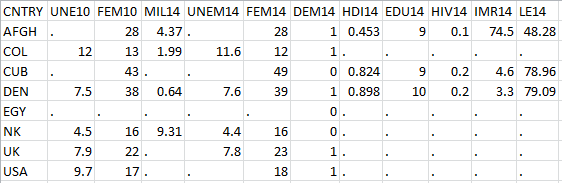
\includegraphics[width=\textwidth]{images/datawide5a}
	\vspace{1em}
	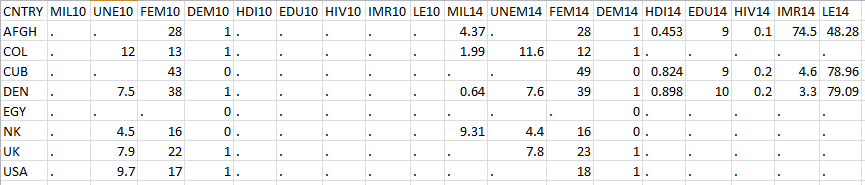
\includegraphics[width=\textwidth]{images/datawide5b}
}


\frame{
	\frametitle{Activity Answer: Long Format}
	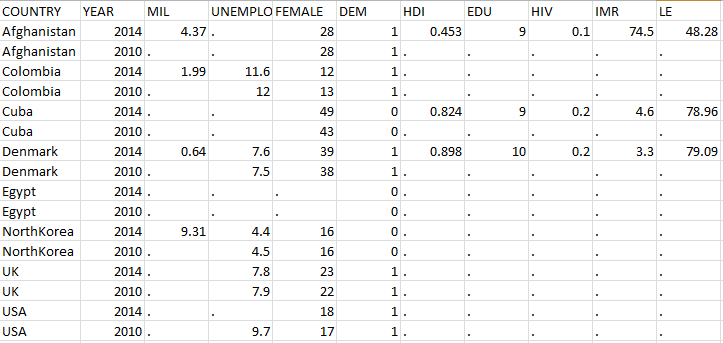
\includegraphics[width=\textwidth]{images/datalong5}
}


\end{document}
